\documentclass[twoside,openright,titlepage,numbers=noenddot,headinclude,%
               footinclude=true,cleardoublepage=empty,abstractoff,BCOR=5mm,%
               paper=a4,fontsize=11pt]{book}

\usepackage{scrextend}  % for addmargin command
\usepackage{graphicx}
\usepackage[usenames, dvipsnames]{color}

% To add line number
\usepackage{lineno}

\usepackage{comment}

\usepackage{epigraph}

% for <bra> <ket> notation 
\usepackage{braket}

% for degree symbol (https://tex.stackexchange.com/questions/384873/what-is-the-degree-symbol)
\usepackage{siunitx}

% for highligted tables
\usepackage{tabularx}
\usepackage{colortbl}
\usepackage{hhline}

% packages for todonotes
\usepackage[colorlinks]{hyperref}
\usepackage[table]{xcolor}
\usepackage[colorinlistoftodos]{todonotes}
% \usepackage{menukeys}

\usepackage{url}

\usepackage[backend=bibtex,style=numeric,sorting=none]{biblatex}
\addbibresource{ThesisBibliography.bib}


\usepackage{imakeidx}
\makeindex

\usepackage[acronym,toc,nomain,nonumberlist]{glossaries}
\makeglossaries

%
%	define all acronyms
%
\newacronym{sm}{SM}{Standard Model}
\newacronym{lhc}{LHC}{Large Hadron Collider}
\newacronym{hep}{HEP}{High Energy Physics}

 

\begin{document}
 \linenumbers
 \pagenumbering{roman}
 \pagestyle{plain}

% Front pages =================================================================
 % \begin{titlepage}
	\begin{addmargin}[-1cm]{-3cm}
    \begin{center}
        \large
        {\Large \textsc{University of Delhi}}\\[1ex]
        Department of Physics \& Astrophysics\\

        \vfill

        PhD Thesis\\ \vskip1cm
        \rule{14cm}{0.4pt} \\ \bigskip
        % \begingroup
            % \Large
            {\color{Maroon}{{\LARGE{S}}EARCH {\LARGE{F}}OR {\LARGE{N}}EW {\LARGE{P}}HENOMENA {\LARGE{I}}N {\LARGE{H}}IGH {\LARGE{E}}NERGY {\LARGE{I}}NTERACTIONS}} \\ \bigskip
            % \color{Maroon}\spacedallcaps{\myTitle} \\ \bigskip
        % \endgroup
        %\spacedlowsmallcaps{\mySubtitle} \\ \bigskip
        \rule{14cm}{0.4pt}\\ \vskip1cm
        by \textsc{Ram Krishna Sharma}

        \vfill
        \vfill
        \vfill

        \hfill Advisor: Dr. \textsc{Md. Naimuddin}\\
        %\hfill April 2017
    \end{center}
    \vspace{-3.5cm}
\includegraphics[width=0.35\textwidth]{figures/logo_du.jpg}
  \end{addmargin}
\end{titlepage}
 \listoftodos
  % \cleardoublepage \begin{center}
\textbf{\LARGE Declaration}
\end{center}
\vspace{1.5cm}
This thesis describes work done by the candidate during his tenure as Ph.D. student at the Department of Physics and Astrophysics, University of Delhi, Delhi, India under the supervision of Dr. Md. Naimuddin. The work reported in this thesis is original and it has not been submitted earlier for any degree to any university. 
\vfill
{\flushleft Candidate} \hspace{4cm} \dotfill \\
{\flushright {\textbf{Ram Krishna Sharma}}}

\vfill
{\flushleft Supervisor} \hspace{4cm} \dotfill \\
{\flushright{\textbf{Dr. Md. Naimuddin}}}

\vfill
{\flushleft Head of Department} \hspace{2.5cm} \dotfill \\
{\flushright {\textbf{Prof. Sanjay Jain}}}
\vfill
  % \cleardoublepage%\vspace{1.5cm}
%
\begin{tabular}{l}

\includegraphics[scale=0.7]{figures/logo_du.jpg}
\end{tabular}
%
\hspace{3cm}
\begin{tabular}{r}
 \\
 \\
\color{blue} \textbf{Department of Physics  and Astrophysics} \\
 \\
\textbf{University of Delhi} \\
 \\
\textbf{Delhi-110007, India} \\
 \\
 \\
 \\
 \\
Date: ...................................  
\end{tabular}
%
\vspace{4cm}
\begin{center}
\textbf{\LARGE Certificate of Originality}
\end{center}
\vspace{1.5cm}
%
The research work embodied in this thesis entitled~``\textbf{Search For New Phenomena In High Energy Interactions}'' has been carried out by me at the \textbf{Department of Physics and Astrophysics}, University of Delhi, Delhi, India. The manuscript has been subjected to plagiarism check by \textbf{Turnitin} software. The work submitted for consideration of award of Ph.D. is original. \\
\begin{tabular}{cc}
 & \\
 & \\
 & \\
 & \\
 & \\
 & \hspace{9cm} ............................................................. \\
 & \hspace{9cm} \textbf{Ram Krishna Sharma} \\
 & \hspace{8.5cm} Name and Signature of the Candidate
\end{tabular}
  % \cleardoublepage\begin{center}
\textbf{\LARGE Student Approval Form}
\end{center}
\vspace{1cm}
%
%
%
\begin{tabular}{|l|p{12cm}|} \hline
 & \\ [-1em]
Name of the Author & {\bf Ram Krishna Sharma}\\ \hline
 & \\ [-1em]
Department & Department of Physics and Astrophysics\\ \hline
 & \\ [-1em]
Degree &  Doctor of Philosophy \\ \hline
 & \\ [-1em]
University & University of Delhi \\ \hline
 & \\ [-1em]
Guide & Dr. Md. Naimuddin \\ \hline
 & \\ [-1em]
Thesis Title & Search For New Phenomena In High Energy Interactions\\ \hline
 & \\ [-1em]
Year of Award & \\ \hline
\end{tabular}
%
%
%
\vspace{1cm}
%
%
%
\begin{center}
\textbf{Agreement} \\
\end{center}
\vspace{0.5cm}
\begin{enumerate}
\item I hereby certify that if appropriate, I have obtained and attached hereto a written permission/statement from the owner(s) of each third party copyrighted matter to be included in my thesis/dissertation, allowing distribution as specified below.
\item I hereby grant to the university and its agents the non-exclusive license to archive and make accessible, under the conditions specified below, my thesis/dissertation, in whole or in part in all forms of media, now or hereafter known. I retain all other ownership rights to the copyright of the thesis/dissertation. I also retain the right to use in future works (such as articles or books) all or part of this thesis, dissertation, or project report.
\end{enumerate}
\vspace{1cm}
%
%
%
\textbf{Conditions:} \\
\vspace{1cm}
\begin{tabular}{|p{10cm}|p{5cm}|} \hline
 & \\ [-1em]
1. Release the entire work for access worldwide & \\ \hline
 & \\ [-1em]
2. Release the entire work for \lq My University\rq only for: & \\ 
~\hspace{2cm}~\begin{tabular} {c} 1 Year \\ 2 Year \\ 3 Year \end{tabular} &  \\ 
and after this time release the work for access worldwide. &  \\ \hline
 & \\ [-1em]
\end{tabular}

  % \cleardoublepage\begin{tabular}{|p{10cm}|p{5cm}|}
 & \\ \hline
 & \\ [-1em]
 3. Release the entire work for \lq My University\rq  only while at the same time releasing the following parts of the work (e.g. because other parts relate to publications) for worldwide access: &  \\
\begin{enumerate} \item[a)] Bibliographic details and Synopsis only \item[b)] Bibliographic details, synopsis and the following chapters only \item[c)] Preview/Table of Contents/24 page only \end{enumerate} & \\ \hline
 & \\ [-1em]
4. View Only (No Downloads) (worldwide) & \\ \hline
\end{tabular}
%
%
%
\begin{tabular}{c}
 \\
 \\
 \\
\end{tabular}
%
%
%
\begin{tabular}{p{7cm}p{8cm}}
 & \\
 & \\
 & \\
 & \\
 & \\
 & \\
 & \\
 & \\
 & \\
........................................... & \hspace{2cm} ....................................................... \\
Signature of the Scholar & \hspace{2cm} Signature and seal of the Guide \\
 & \\
 & \\
 & \\
Place: ......................... & \\
 & \\
 & \\
Date: ......................... &
\end{tabular}

  % \cleardoublepage\begin{center}
\vspace*{6cm}
\Huge
	\textbf{\textit{Dedicated To \\My Loving Parents }}
\end{center}
  % \cleardoublepage% Acknowledgements ============================================================

%\pdfbookmark[1]{Acknowledgments}{acknowledgments}
\chapter*{Acknowledgments}

As the saying goes, good premises do not entail good stories. 
  % \cleardoublepage %\pdfbookmark[1]{Abstract}{Abstract}
\chapter*{Abstract}

In the Standard Model (SM) of particle physics, masses for the particles are generated by the Higgs mechanism, which requires the existence of a spin-0 particle called the Higgs boson. In July 2012, a new Higgs like particle is discovered with mass 125-126 GeV at the LHC. This may be the long sought Higgs boson of the standard model (SM), which was proposed in 1960s, or one of the Higgs bosons beyond the SM. For example, super-symmetric theories, little-Higgs models, and other extended Higgs sector such as the two-Higgs-doublet model (2HDM) all contain a multitude of neutral as well as charged Higgs bosons. Because, the current data still contain large uncertainties that these various extensions of the SM cannot be confirmed or ruled out decisively. So, It is important to at-least constraint the various couplings of the Higgs boson, based on the signal strength of all decay channels of the Higgs boson. One of the most useful constraints from the global fitting of the Higgs boson couplings is the one to a pair of W/Z bosons. The current data constrain
	\begin{equation}
	C_v = \frac{g_{hWW}}{g_{hWW}^{SM}}=0.96^{+0.13}_{-0.15}
	\end{equation}
The central value is close to 1, which means that the observed Higgs boson leaves only little room for the existence of another Higgs boson or some unknown unitarity violation (UV) physics responsible for the electroweak symmetry breaking (EWSB). If $C_v$ is exactly equal to 1, it means that the observed Higgs boson will completely account for the EWSB. We do not need another Higgs boson, or if it exists it has nothing to do with the EWSB.

If the hWW coupling is less than its SM value, there must be something heavier, could be as heavy as a few TeV, to complete the EWSB. 
In particular, through proton-proton collisions it is expected to shed light on the mechanism responsible for electroweak symmetry breaking. 

In the SM of particle physics, masses for the particles are generated by the Higgs mechanism, which requires the existence of a spin-0 particle called the Higgs boson. This particle is discovered now at approx. 125 GeV but it is not sure that it is the Higgs boson which is responsible for the EWSB.

It is possible that the Higgs boson does not exist. In the SM without Higgs boson, the tree level amplitude for longitudinal vector boson scattering $V_LV_L\rightarrow V_LV_L$ violates unitarity at a centre-of-mass energy of 1.2 TeV. New physics, perhaps accompanied by new particles, must appear at or before this scale. It will therefore be crucial to measure vector boson (W or Z) scattering up to the highest possible energies either as a search for the new physics or as confirmation that our understanding of any new physics found in other channels is correct.


  % \pagestyle{headings}
  % \cleardoublepage%\include{frontback/toc}
   % \tableofcontents 
   % \listoffigures 
   % \listoftables
  % Content =====================================================================
  \pagenumbering{arabic}
  % \cleardoublepage
  % \chapter{Introduction}

Particle physics is a modern name for the centuries old effort to understand
the basic laws of physics. -- Edward Witten


Everybody is excited to know about the behaviour of nature around us, e.g. we are standing on earth but where the earth is standing, how it comes into existence, why there are lots of stars, and so on. These are the general questions asked by every human being, and the fundamental physics provides the answer. If we would like to understand it deeper and deeper, it will lead us to the particle physics. As the name infers it deals with the particles (the fundamental particles). However, the question is that how these fundamental particles will give insight into our universe? The answer is that in early universe there are only particles and if we go near the event horizon, then there was only quark gluons plasma. To verify these things, we cannot go back to the early universe, but we can probe them using the high energy colliders to know their behaviour.

One of best model that explains the world around us is the Standard Model (SM). With the discovery of the Higgs boson \cite{Chatrchyan:2012xdj} in 2012 it was complete. However, even now many questions remain unanswered by the SM. List of few questions are:

\begin{itemize}
\item How neutrino get its mass and what is its mass hierarchy? 
\item Why there are only three generations of leptons and quarks? 
\item Why the third generation is too much heavy as compared to other two generations?
\end{itemize}

Now there are two ways to answer these questions. First is to go for another new theory or a model like SUSY, string theory, and others. Another way is to understand the SM profoundly and look for the possible extensions of SM. One of the possible ways is to look for WW scattering. As the Higgs boson unitrize the WW scattering amplitude, so its one of the best path to look for SM deviation.

\begin{itemize}
\item Non-abelian nature => QGC in addition of trilinear gauge coupling.
\item SM includes three types of GGC.
    \item $W^+W^-W^+W^-$
    \item $W^+W^-ZZ$
    \item $W^+W^-\gamma \gamma$
\item ZZZZ vertex is not persent in SM but it is present at tree level via exchange of Higgs boson.
\item $\gamma \gamma ZZ$ vertex is only produced at loop level in SM.
\item Trilinear and quartic couplings probe different aspect of the weak interactions.
    \item Trilinear coupling test the non-abelian nature of SM
    \item Quartic coupling probe the EWSB.
\end{itemize}

\begin{itemize}
\item Heavy vector boson $W^{\pm}$ and $Z$ acquire there mass and longitudinal polarization state through spontaneous EWSB.
\item The mechanism for EWSB must regulate $\sigma(V_LV_L \rightarrow V_LV_L )$ to restore unitarity above $\approx$ 1-2 TeV.
    \item cross-section attenuated to a linear growth by the quartic gauge by the quartic gauge self coupling.
    \item a light SM higgs boson exactly cancels increase for large s (for HWW coupling).
\end{itemize}

\section{Outline and Contributions}


Part-1 of this thesis is dedicated to the CMS detector.

Part-2 consists of my GEM work.

Part-3 consists of physics analysis.

\begin{itemize}
\item Introduction and motivation     
\item What is particle physics?     
\item Introduction to particle physics?
\item Introduction to GEM detectors 
\item Motivation for HEP detectors
\item LHC and CMS 
\item GEM detectors 
\item GEM Hardware work
\item GEM test beam work
\item Physics of WW scattering  
\item Physics Analysis details     
\item Basic experimental techniques     
\item MC generation and study     
\item Data/MC comparison study    
\item Background estimation     * TMVA     * Limits for aQGC and Charged Higgs *
\item Summary and outlook
\end{itemize}

\section{Summary of chapters}

This is an outline of what went into each chapter. **Chapter 1** gives a
background on duis tempus justo quis arcu consectetur sollicitudin.  **Chapter
2** discusses morbi sollicitudin gravida tellus in maximus.  **Chapter 3**
discusses vestibulum eleifend turpis id turpis sollicitudin aliquet.  **Chapter
4** shows how phasellus gravida non ex id aliquet. Proin faucibus nibh sit amet
augue blandit varius.

  % \chapter{Introduction}

An understanding of how the world is put together requires a theory of how the elementary particles of matter interact with one another[@paper:ScientificAmericantHooft]. There are many theories to explain this interaction but the theory that explains best is the sm. This is called as Model because it is based on some of experimental inputs. An important problem in physics is to understand the ultimate constituents of matter and the fundamental interactions that occur amongst them; it is of equal importance to establish whether these interactions are, in reality, different manifestations of a single underlying (or unified) interaction which is yet to be discovered. The weak and electromagnetic interactions are unified in the electroweak theory of the SM at an energy scale already attained at particle accelerators around the world. The electroweak SM and the QCD, describing the strong interaction together forms the complete SM of the electroweak and strong interactions. However, there are strong reasons which suggest that the SM is not the ultimate theory and there must exist some phenomena beyond SM \cite{paper:ScientificAmericanChrisQuiggEPF} \cite{article:PAdventure}

\section{Standard Model as Gauge theory}
% The concept of gauge invariance is fundamental in the construction of the Standard Model of strong, weak and electromagnetic interactions of elementary particles. The gauge principle prescribes that, given the gauge symmetry group and the transformations of the fields, the quantum field theory is uniquely defined [@book:CoughlanDodd].

QED is a local gauge theory because the Lagrangian function that describes it remains unchanged by the following local gauge transformation of the electron field $\psi(x)$ and the photon field $A_\mu(x)$ at all space-time point x:
    \begin{eqnarray}
    \psi(x) & \rightarrow & e^{ie\Lambda(x)}\psi(x), \nonumber \\
    A_\mu(x) & \rightarrow & A_\mu(x) + \frac{\partial \Lambda(x)}{\partial x_\mu}, \nonumber
    \end{eqnarray}
with arbitrary $\Lambda(x)$, where e is the electron-photon coupling (other charged spin-$\frac{1}{2}$ fields transform similarly to $\psi$). The photon field plays an intrinsic part; there could be no local gauge invariance without it. Hence if we take the postulate of this local gauge invariance for spin-$\frac{1}{2}$ particles as a starting point, the existence of gauge boson is required and in fact their coupling to fermions is specified, too. For exact gauge invariance the gauge bosons must be massless.

The phase factor $e^{i\Lambda(x)}$ belong to the symmetry group $U(1)$ of unitarity transformations in one dimension. The generalization of {qed} to other forces is made by looking for other possible symmetry groups and using them as the basis of more general gauge transformations. 
        
For example, we may choose to regard the electron and neutrino as a doublet $(\nu_e,e)$, i.e. as two members of the same family, since both are light spin-$\frac{1}{2}$ particles. We can then describe this doublet by a two component field $\psi = (\psi_\nu,\psi_e)$ and introduce gauge transformations where $\Lambda$ is a $2\times 2$ hermitian matrix operating on $\psi$.  We can put the other leptons and the quarks, too, in doublets $(\nu_\mu,\mu),(\nu_\tau,\tau),(u,d),etc.$ and subject them to similar gauge transformations. These transformations are much more than phase factors, since the off-diagonal elements of $\Lambda$ can change one member of a doublet into the other; they belong to the symmetry group SU(2) of unitary unimodular transformations in two dimensions. Local gauge invariance in this case requires the introduction of three massless spin-1 gauge bosons $W^+,W^-$ and $W^0$. If this is combined with a simultaneous U(1) symmetry (bringing one more gauge boson $B^0$), we get the $SU(2)_L\times U(1)$ Glashow-Salam-Weinberg theory of electroweak interactions [article:weinberg]. The gauge bosons can not all be massless, experiment excludes this, so the symmetry can not be exact. The symmetry is broken spontaneously, in a way that retains renormalizability; the result is one massless gauge boson $\gamma$ (made from a linear combination $W^0sin\theta_w +B^0cos\theta_w$) plus three massive gauge bosons $W^+, W^-$ and $Z^0$ (the orthogonal combination $W^0cos\theta_w - B^0sin\theta_w$). The angle $\theta_w$ is a parameter of this unified electroweak theory.

The subscript L on $SU(2)_L$ above indicates that the $SU(2)$ gauge transformations operate only on left-handed particles. This is because processes like beta-decay are observed to involve quarks and leptons with left-handed spins relative to their motions. The remaining right-handed spins relative to their motions singlets that do not change under $SU(2)_L$ gauge transformations; for anti-quark and anti-leptons, interchange L and R. The first-generation spin-$\frac{1}{2}$ particles can be classified in doublet and singlet representations of $SU(2)_L$ as follows:
    \begin{eqnarray}
    (u_L,d_L),(\nu_{eL},e_L),\bar{u}_L,\bar{d}_L,\bar{e}_L, \nonumber \\
    (\bar{d}_R,\bar{u}_R),(\bar{e}_R,\bar{\nu}_{eR}),u_R,d_R,e_R.   \nonumber
    \end{eqnarray}
There is no right-handed neutrino state here; there is no need for such states to exist if the neutrino is massless. Thus we have 15 left-handed (and 15 right-handed) fermion states in each generation counting three colors for each quark flavor, in this gauge theory of electroweak interactions.

% <!-- %In chiral theories, where gauge bosons have different couplings to left and right handed fermion states a new problem arises- typically for the interaction of three gauge bosons via a closed loop of fermions as shown in figure
% %add figure
% %When the L and R fermion couplings are unequal at one (or three) of the vertices, as is the case in the standard electroweak theory -->

In strong interactions since each quark has three possible colors, we can describe any particular quark flavor by a three-component field $\psi(x)=[\psi(red,x),\psi(blue,x),\psi(green,x)]$ and can consider local gauge transformations where $\Lambda(x)$ is a $3\times 3$ hermitian matrix operating on $\psi$. The transformation can change the color; they belong to the symmetry group SU(3). To achieve local gauge invariance in this case requires the introduction of eight massless gauge bosons which carry pairs of color labels and are known as gluons. This gauge theory is known as {qcd}. Combining with the electroweak interaction gives an $SU(3)\times SU(2) \times U(1)$ gauge invariant theory of the strong and electroweak forces, commonly called the Standard Model.

With each of these gauge groups $(SU(3),SU(2)$ and $U(1))$ there is associated a characteristic coupling strength $\alpha_3,~\alpha_2,~\alpha_1$ analogous to the fine-structure constant $\alpha$ of electrodynamics. They are generally called the running couplings because their numerical values change logarithmically with the energy scale of the interaction due to renormalization.

These renormalizable gauge theories allow the presence of spin 0 (scalar) particles, too [article:higgs]. The usual formulation of the Standard Model requires at least one of these, the Higgs scalar boson, arising from the mechanism for spontaneously breaking the $SU(2)\times U(1)$ electroweak symmetry and giving masses to the weak gauge bosons and to the leptons and quarks. This mechanism is a vital part of the SM [@book:barger] [@book:Braibant] [@book:FrankClose] [@book:Griffiths].


\section{Introduction2}
An understanding [@Chatrchyan:2012xdj] of how the world is put together requires a theory of how the elementary particles of matter interact with one another [@paper:ScientificAmericantHooft]. There are many theories to explain this interaction but the theory that explains best is the SM. This is called as Model because it is based on some of experimental inputs. An important problem in physics is to understand the ultimate constituents of matter and the fundamental interactions that occur amongst them; it is of equal importance to establish whether these interactions are, in reality, different manifestations of a single underlying (or unified) interaction which is yet to be discovered. The weak and electromagnetic interactions are unified in the electroweak theory of the SM at an energy scale already attained at particle accelerators around the world. The electroweak SM and the QCD, describing the strong interaction together forms the complete SM of the electroweak and strong interactions. However, there are strong reasons which suggest that the SM is not the ultimate theory and there must exist some phenomena beyond SM [@paper:ScientificAmericanChrisQuiggEPF] [@article:PAdventure].  

Presently, the most profound problem of the standard model is to find out the reason behing the spontaneous symmetry breaking\footnote{The spontaneous symmetry breaking takes place when a system, that is symmetric with respect to some symmetry group, goes into a vacuum state that is not symmetric. At this point the system no longer appears to behave in a symmetric manner}. This leads to solution of many problem that we are facing like the it gives the ideas about the mass generation, it solves the problem of unitarity in vector-boson scattering, etc. If we do not break the symmetry of system then all the force carrieres for all interaction should be massless but it is not observed in the nature. Thus, nature suggest that symmetry should be broken spontaneously. So, In next section I am going to describe brefily that how the spontaneous symmetry breaking solves the problem of mass generation. This is known as the Higgs mechanism [@article:higgs] [@article:Englert] [@article:kibble].

\section{Brief Introduction to Higgs mechanism}
This is brief intro to higgs.

Electroweak symmetry breaking and the Higgs mechanism: [@article:LEPtoLHC] [@article:abd][@article:tasi]
The Higgs part
    \begin{equation}
    L_H=(D_{\mu}\Phi)^{\dagger}(D^{\mu}\Phi)-V(\Phi)
    \end{equation}
of the SM lagrangian extends the experimentally well established particle content of the SM by the complex scalar SU(2) doublet $\Phi = (\phi^{+},\phi^0)^T$ of weak hypercharge $Y_{w,\Phi}=1$, so that $\phi^{+}$ carries charge +e and $\phi^0$ is neutral. In toal $\Phi$ involves four degree of freedom. The self-interaction of $\Phi$ is described by the potential
    \begin{equation}
    V(\Phi)=-\mu^2(\Phi^{\dagger}\Phi)+\frac{\lambda}{4}(\Phi^{\dagger}\Phi)^2,
    \end{equation}
Here, the term $\lambda > 0$ ensures that the potential is bounded form below. Here we need to generate masses for the three gauge bosons $W^{\pm}$ and Z but the photon should remain massless. Therefore, we needs at least 3 degree of freedom for the scalar fields. The simplest choice is a complex SU(2) doublet of scalar field $\phi$
    \begin{equation}\label{mat2}
    \Phi=
        \begin{bmatrix}
        \phi^+  \\
        \phi^0  \\
        \end{bmatrix}
    =\frac{1}{\sqrt{2}}
        \begin{bmatrix}
        \phi_1 + i\phi_2    \\
        \phi_3 + i\phi_4    \\
        \end{bmatrix}
    \end{equation}
where $\phi_i$ are 4 real scalar fields (4 degree of freedom). The lagrangian is invariant under the local gauge transformations \footnote{The concept of gauge invariance is fundamental in the construction of the Standard Model of strong, weak and electromagnetic interactions of elementary particles. The gauge principle prescribes that, given the gauge symmetry group and the transformations of the fields, the quantum field theory is uniquely defined [@book:CoughlanDodd]}
    \begin{equation}
    \Phi (x) \rightarrow \Phi(x)`=e^{i\alpha_i(x)\tau_i /2}\Phi(x)
    \end{equation}
where $\tau_i$ are Pauli matrices and $\alpha_i(x)$ are transformation parameters.
Now the product
    \begin{equation}\label{mat1}
    \Phi{\dagger}\Phi=
        \begin{bmatrix}
        \phi^{+*}   &   \phi^{0*} \\
        \end{bmatrix}
        \begin{bmatrix}
        \phi^+  \\
        \phi^0  \\
        \end{bmatrix}
    =\phi^{+*} \phi^+ + \phi^{0*}\phi^0
    =\frac{1}{2}(\phi^2_1+\phi^2_2+\phi^2_3+\phi^2_4)
    =\frac{1}{2}\phi_i \phi^i
    \end{equation}
    
For $\mu^2<0$, the potential $V(\Phi)$ has a minimum at
    \begin{equation}
    \Phi^{\dagger}\Phi = -\frac{\mu^2}{2\lambda}=\frac{v^2}{2}
    \end{equation}
from equation (\ref{mat1}) we can know that there is an infinite number of possible solutions of this equation. To preserve electric charge conservation ($U(1)_{QED}$ symmetry), this non zero vacuum expectation value should not be reached in the charged direction. A conveninent choice of the neutral direction is $\phi_1 = \phi_2 = \phi_4 = 0$. So, the equation (\ref{mat2})
    \begin{equation}
    \Phi=\frac{1}{\sqrt{2}}
        \begin{bmatrix}
        0   \\
        \phi_3  \\
        \end{bmatrix}
    \end{equation}
Therefore, the neutral component ($\phi_3$) of the doublet field $\Phi$ develops a nonzero vacuum expectation value
\begin{equation}
{\Braket\Phi}_0 = \Braket{0|\Phi|0}=\frac{1}{\sqrt{2}}
        \begin{bmatrix}
        0   \\
        v   \\
        \end{bmatrix}
        with~
        v=-
        \begin{bmatrix}
        \frac{\mu^2}{\lambda}
        \end{bmatrix}
        ^{1/2}
\end{equation}
Now by using the unitarity gauge\footnote{It removes the unphysical degree of freedom} means of proper gauge transformation of the field we get
    \begin{equation}
    \Phi (x)=\frac{1}{\sqrt{2}}
        \begin{bmatrix}
        0   \\
        v+h(x)  \\
        \end{bmatrix}
    \end{equation}
With $\Phi(x)$ we can expand kinetic term $D_\mu \Phi)^{\dagger} (D_\mu \Phi)=|D_\mu \Phi|^2$ of lagrangian
    \begin{eqnarray}\label{mat3}
    |D_{\mu} \Phi|^2 & = & |(\partial_{\mu}-ig_2\frac{\tau_a}{2}W^a_{\mu}-ig_1 \frac{Y_H}{2}B_{\mu})\Phi|^2 \nonumber \\
            & = & \frac{1}{2}(\partial_\mu H)^2+\frac{1}{8}g^2_2(v+H)^2|W^1_{\mu}+iW^2_\mu|^2+\frac{1}{8}|g_2W^3_\mu-g_1B_\mu|^2
    \end{eqnarray}
Lets define the new fields $W^{\pm}_\mu$ and $Z_\mu$ [$A_\mu$ is the field orthogonal to $Z_\mu$]:
\begin{equation}
    W^{\pm}=\frac{1}{\sqrt{2}}(W^1_\mu \mp iW^2_\mu),~Z_\mu=\frac{g_2W^3_\mu-g_1B_\mu}{\sqrt{g^2_2+g^2_1}},~A_\mu=\frac{g_2W^3_\mu+g_1B_\mu}{\sqrt{g^2_2+g^2_1}}
\end{equation}
Now pic the term from equation (\ref{mat3}) which are bilinear in the fields $W^\pm,Z,A$:
    \begin{equation}
    M^2_wW^+_\mu W^{-\mu},~\frac{1}{2}M^2_z Z_\mu Z^\mu,~and~\frac{1}{2}M^2_AA_\mu A^\mu
    \end{equation}
Then we noted that W and Z boson have acquired masses, while the photon is still massless
    \begin{equation}
    M_w=\frac{1}{2}vg_2,~M_z=\frac{1}{2}v\sqrt{g^2_2+g^2_1},~M_A=0
    \end{equation}
So, by spontaneously breaking the symmetry, three Goldstone bosons have been absorbed by the $W^\pm$ and Z boson to form their longitudinal components and to get their masses. Since the U(1) symmetry is still unbroken, the photon which is its generator, remains massless.


Now we established that the Higgs mechanism generates the mass for the vector boson. So, now it following the nature. But for the Higgs mechanism to be validated Higgs boson should be found experimentally. In July 2012, we found a higgs like boson. But, is it the Higgs of SM or someting else we can say now because of the uncertainty \& statistical error involved in the present analysis. 

So, What are the possible ways to investigate it?

Basically there are two possible ways to investigate it. First, we should try to study the coupling of the Higgs boson with different particle (top quark is the best candidate). Secondly, we should try to study the vector boson scattering.

  % \include{chapters/Introduction3}
  \chapter{The LHC Machine}

The famous quote "history repeats itself" \acrlong{gcd} applies well to the high energy physics (HEP). The starting point of experimental high energy physics is the Rutherford $\alpha$-particle scattering, and even now we are doing the same thing just the method changed from "natural accelerator" to the "man-made" accelerator that can accelerate particles \acrshort{gcd} with the velocity close to the speed of light. The design and working of accelerator changed a lot over a period in going from MeV to GeV and now to the multi-TeV range. Now, these machines are not only used in HEP \acrfull{lcm} experiments, but it went to treat human beings like cancer therapy, \index{radioisotope} production,  to the industry for \index{uses} like material processing, sterilisation, security scan, water treatment, and many more. 



Below table is taken from \cite{Schoerner-Sadenius2015, LHC-parameters-2016, LHC-tdr}. THis is ram.


\begin{tabularx}{\textwidth}{|l c c|}
    \hhline{---}
    {\bf } \cellcolor[gray]{.8}& {\bf Injection} \cellcolor[gray]{.8}& {\bf Collision}\cellcolor[gray]{.8} \\
    \hhline{---}
    {\bf Proton energy (GeV)} & 450 & 6500\\
    \hhline{---}
    {\bf Circumference (m)} &  26658.883 & \\
    \hhline{---}
    {\bf Particles/bunch ($10^{11}$)}& 1.18 &  \\
    \hhline{---}
    {\bf Number of bunches} &   2076 &  \\
    \hhline{---}
    {\bf Bunch distance (ns)}   &  25 &   \\
    \hhline{---}
    {\bf Bunch length (ns)} &    1.05 & \\
    \hhline{---}
    {\bf Beam current (mA)} &   584 &   \\
    \hhline{---}
    {\bf Norm. emittance (x and y) ($\mu$ mrad)}  &  3.5 &  2.6 \\
    \hhline{---}
    {\bf Stored energy per beam (MJ)}   &  23.3 &  362 \\
    \hhline{---}
    {\bf Rms beam size at IP1 and IP5 ($\mu$ m)}  &  375 &  17 \\
    \hhline{---}
    {\bf Rms beam size at IP2 and IP8 ($\mu$ m)}  &  280 &  71 \\
    \hhline{---}
    {\bf Peak luminosity ($cm^{-2}s^{-1}$)}   &   & 1.1 $\times ~ 10^{34}$  \\
    \hhline{---}
    {\bf Average luminosity lifetime ($\tau$) (hours)} &    &   24 \\
    \hhline{---}
    {\bf Average mean pile-up}  &   &   27  \\
    \hhline{---}
\end{tabularx}
% Ref: \url{https://lhc-commissioning.web.cern.ch/lhc-commissioning/performance/2016-performance.htm]}


  \section{CMS Detector}
  \section{Data Taking}
  % \chapter{WW Scattering}
\section{Introduction}
When two W-boson interacts directly it is known as WW scattering. It is shown in figure \ref{wwscattering1}.
\begin{figure}[htb]
	\begin{center}
		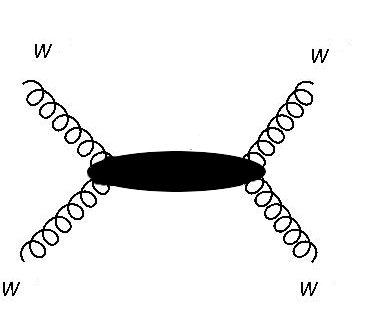
\includegraphics[width=8.0cm,height=6cm]{figures/VBS/H-mediated.png}
		\caption{WW scattering process}
		\label{wwscattering1}
	\end{center}
\end{figure} 
In figure black box represent that we do not know the process by which it is happening. It may be the Higgs which is responsible for it or may be something else which is beyond standard model scenario.
\section{Motivation for WW Scattering}
In July 2012, a new Higgs like particle was discovered with mass $125.7\pm 0.3(stat)\pm 0.3 (syst)$ GeV at the LHC \cite{paper:Higgs2013}. This may be the long sought Higgs boson of the {sm}, which was proposed in 1960s, or one of the Higgs bosons beyond the {sm} predicted by many BSM models. For example, super-symmetric theories, little-Higgs models, and other extended Higgs sector such as the two-Higgs-doublet model (2HDM) all contain a multitude of neutral as well as charged Higgs bosons\cite{paper:13036335v1}. Because, the statistical and systematic uncertainties of current data are still sizable ($\sim20\%$ in the best cases), therefore it is not possible at present to conclude with precision whether this particle is the Higgs boson of the {sm}, nor if new physics is present in the Higgs sector\cite{paper:Higgs2013}.

A well known probe to {ewsb} is the scattering of the longitudinal components of the weak gauge bosons\cite{paper:13036335v1}.% The scattering amplitude with purely gauge contributions grow with energy as $s/m^2_w$, where s is the squared  \gls{com} energy of the $W_LW_L$ system. In the SM with light Higgs boson, the amplitude will be completely unitarized by the Higgs boson. Once $\sqrt{s}$ goes beyond the light Higgs boson mass, the scattering amplitude will no longer grow like $s/m^2_w$. 
The centrality of WW scattering to the exploration of {ewsb} stems from the issue of cancellation of high energy divergences. Any scattering amplitude in a consistent quantum mechanical theory must respect the unitarity, which is equivalent to the conservation of total probability. This implies that no amplitude can indefinitely grow with energy. The reaction which best exemplifies the relationship between unitarity and {ewsb} is the scattering among longitudinally polarized vector bosons. The Feynman diagrams for $W^+W^-\rightarrow W^+W^-$ are shown in Figure \ref{wwscattering} \cite{report:wwscatering}.% The polarization vectors of a transversely/longitudinally (T/L) polarized W boson travelling along the $\hat{z}$ axis are:
\begin{figure}[htb]
	\begin{center}
		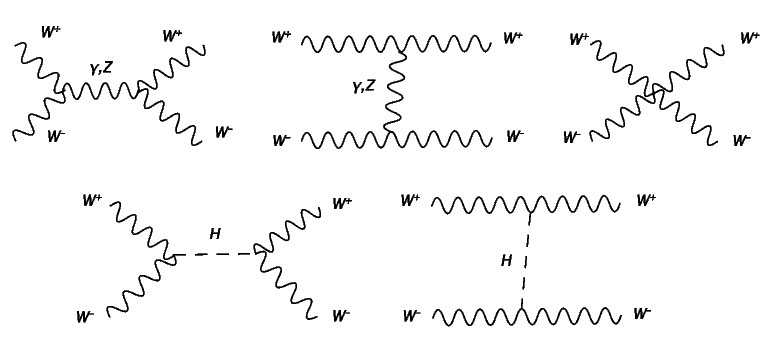
\includegraphics[width=14.0cm,height=8cm]{figures/VBS/wwscattering.png}
		\caption{Vector boson scattering process}
		\label{wwscattering}
	\end{center}
\end{figure} 

%In WW scattering, in the absence of a relatively light Higgs boson, treelevel unitarity is violated at about 1 TeV, therefore either the Higgs must exist or some other mechanism must intervene at about the TeV scale and play same role in taming the divergent behaviour of high energy amplitudes. Hence these processes are the ideal testing ground for the mechanism of EWSB.

\begin{comment}
So, It is important to at-least constraint the various couplings of the Higgs boson, based on the signal strength of all decay channels of the Higgs boson. One of the most useful constraints from the global fitting of the Higgs boson couplings is the one to a pair of W/Z bosons. The current data constrain
	\begin{equation}
	C_v = \frac{g_{hWW}}{g_{hWW}^{SM}}=0.96^{+0.13}_{-0.15}
	\end{equation}
The central value is close to 1, which means that the observed Higgs boson leaves only little room for the existence of another Higgs boson or some unknown  \gls{uv} physics responsible for the  \gls{ewsb}. If $C_v$ is exactly equal to 1, it means that the observed Higgs boson will completely account for the \gls{ewsb}. We do not need another Higgs boson, or if it exists it has nothing to do with the \gls{ewsb}.

If the hWW coupling is less than its \gls{sm} value, there must be something heavier, could be as heavy as a few TeV, to complete the \gls{ewsb}. 
In particular, through proton-proton collisions it is expected to shed light on the mechanism responsible for electroweak symmetry breaking. 

%In the \gls{sm} of particle physics, masses for the particles are generated by the Higgs mechanism, which requires the existence of a spin-0 particle called the Higgs boson. This particle is discovered now at approx. 125 GeV but it is not sure that it is the Higgs boson which is responsible for the \gls{ewsb}.
\end{comment}
It is also possible that the Higgs boson does not exist at all. %In the \gls{sm} without Higgs boson, the tree level amplitude for longitudinal vector boson scattering $V_LV_L\rightarrow V_LV_L$ violates unitarity at a centre-of-mass energy of 1.2 TeV. 
Then, the new physics, perhaps accompanied by new particles, must appear at or before electroweak scale. It will therefore be crucial to measure vector boson (W or Z) scattering up to the highest possible energies either as a search for the new physics or as confirmation that our understanding of any new physics found in other channels is correct \cite{phdThesis:Bruno}.


%%%%%%%%%%%%%%%%%%%%%%%%%%%%%%%%%%%%%%%%%%%%%%%%%%%%%%%%%%%%%%%%%%%%%%%%%%%%%%%%%%%%%%%%%%%%%%%%%%%%%%%%%%%%%%%%%%%%%%%%%%%%%%%%%%%%
\section{WW Scattering at the Large Hadron Collider}
At a hadron collider like {lhc} , WW scattering can occur with virtual W's emitted by the quarks in the hadrons. A W pair in the final state can be produced either through WW scattering diagrams, or through W emission from the partons of the initial hadrons. Figure \ref{wwscat} shows these two types of contributions. Figure \ref{wwscat}(a) represents the genuine WW scattering diagram, whereas Figure\ref{wwscat}(b) shows the ``Bremsstrahlung" diagrams, which would be a background in the study of WW scattering.\cite{book:PhyAtLHCdebjo} 
\begin{figure}[htb]
	\begin{center}
		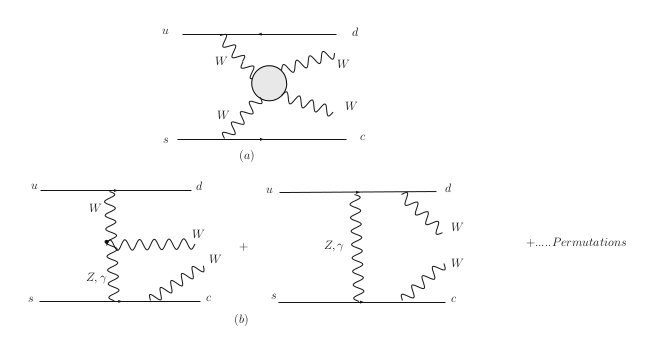
\includegraphics[width=16.0cm,height=8cm]{figures/VBS/ww_scat.png}
		\caption{Main diagram topologies for the process $us \rightarrow cdW^+W^-$}
		\label{wwscat}
	\end{center}
\end{figure} 
Thus to study WW scattering at the LHC, we have to find out the ways of separating the genuine scattering contribution from the other ``Bremsstrahlung" contributions, which is no mean task. 
\begin{comment}
\subsection{Backgrounds}
It is important to understand the first inherent background, and device cuts which may enhance the signal. Generally, the backgrounds in this case are of two types:
\begin{enumerate}
	\item Bremsstrahlung processes - these are processes where the vector bosons are radiated by quark or anti-quark partons, and which do not contribute to VV scattering.
	\item Processes which fake a VV final state.
\end{enumerate}
 The second background is crucial to take care of, otherwise we do not know if we are observing a VV pair in the final state or not.

Background processes are $q\bar{q} \rightarrow W^+W^-X$, $gg \rightarrow W^+W^-X$, $t\bar{t}+jet$, with top decays giving $W^+W^-$ pair. Electroweak-\gls{qcd} process $W^+ +jets$ can mimic the signal when the invariant mass of the two jets is around $m_w$. There is a potential background from \gls{qcd} processes $q\bar{q},gg\rightarrow t\bar{t}X,$  $Wt\bar{b}$ and $(t\bar{t} + jets)$, in which a W can come from the decay of $t$ or $\bar{t}$. W boson pairs produced from the intrinsic electroweak process $q\bar{q}\rightarrow q\bar{q}W^+W^-$ tend to be transversely polarised. 


Compared to the dileptonic channel, the well-known challenge for the semileptonic $W_LW_L$ scattering is the contamination from \gls{qcd} backgrounds. However, the semileptonic channel is still appealing because it yields much more signal events and enables reconstruction of the W momenta and thus important kinematics such as the WW invariant mass.\cite{arXiv:WWscat-WjetTag} 
\end{comment}
\subsection{Signal \& Background Details}
I have started working on WW scattering measurement at the {cms} experiment \cite{paper:JINST:CMSCollaboration}. The {lhc} is currently going through shutdown after running for 3 years at 7 \& 8 TeV centre of mass energy. {cms} experiment collected about $5fb^{-1}$ of data at 7TeV and $20fb^{-1}$ data at 8TeV. The {lhc} is scheduled to start operating at 13 and/or 14 TeV energy form next year. Since the WW scattering measurement prospects will increase considerably at higher energies so we need to be prepared fully to perform this measurement once LHC starts delivering the data. Currently I am working on the development of necessary techniques needed to discriminate the WW signal from the other similar SM backgrounds.\\ {\large \bf Signal :} Since the channel on which I work is $qq\rightarrow qqW_LW_L \rightarrow l\nu jjjj$. So, my signal in first stage contains 2 jets that are coming from hadronic decay of quarks and two longitudinal component of W. And in last stage it contains one lepton, 4 jets (2 coming from hadronic decay of quarks and 2 coming from hadronic decay of $W_L$) and one neutrino which constitute missing energy. Here, lepton includes electron and muon.\\{\large \bf Background :} The processes which can fake the final state are known as background. It is important to understand the first inherent background, and device cuts which may enhance the signal. Generally, the backgrounds in this case are of two types:
\begin{enumerate}
	\item Bremsstrahlung processes - these are processes where the vector bosons are radiated by quark or anti-quark partons, and which do not contribute to VV scattering.
	\item Processes which fake a VV final state.
\end{enumerate}
 The second background is crucial to take care of, otherwise we do not know if we are observing a VV pair in the final state or not.
All possible backgrounds are:
	\begin{enumerate}
		\item {\bf W+Jets :} Most dominating background. W decays to $l\nu $
		\item {\bf Drell-Yan $Z/\gamma*$+ Jets :} $Z/\gamma*$ decays to $l^+l^-$ and we mismeasure one l because of acceptance or inefficiency effects, gives missing energy.
		\item {\bf WW :} This is irreducible background for analysis.
		\item {\bf WZ :} Z decays to $l^+l^-$ and we mismeasure one $l$ giving missing energy. And W decays hadronically.
		\item {\bf ZZ :} One Z decays hadronically and another leptonically and we miss one $l$.
		\item {\bf $t\bar{t}$ Jets :} Top quark always decays to one b quark and one W boson. So, $t\bar{t} \rightarrow bWbW \rightarrow bl\nu bl\nu$, if we mismeasure one $l$ and and b quark forms jet.
		\item {\bf Single top production :} Here $t\rightarrow bW \rightarrow bl\nu $, and 3 fake jet is reconstructed or we get some form ISR or FSR.
	\end{enumerate}

\subsection{Separating Signal form various Background}
The central issue for the experimental detection of WW scattering is to separate the signal among all the various backgrounds. The signal is the {vbf} diagrams, each of the initial quarks radiates a W/Z boson, which further scatters into the final state W/Z bosons. The unique feature of this process is that the scattered quark is very energetic, carrying almost all the energy of the incoming quark and very forward. Furthermore, if we demand the leptonic decays of the W and Z bosons, there will be very little hadronic activities in the central rapidity region. Therefore, the signature includes
	\begin{enumerate}
		\item the appearance of two energetic forward jets with large spatial separation, and 
		\item the leptonic decay products of the W or Z bosons are enhanced at the large invariant mass region.
	\end{enumerate}
Based on these features we can start the analysis by imposing the following experimental cuts for the two jets in selecting the VBF events:
	\begin{itemize}
		\item Two tagging jets $j_1,j_2$ with \begin{equation} 2<|\eta|<5,~ p_T>25GeV,~E>340GeV,~and~\eta_{j1}.\eta_{j2}<0 \end{equation} Where $\eta$ is the rapidity of either jet,\\ $p_T$ is the transverse momentum,\\ E is the energy, \\ $\eta_{j1} ~ \& ~ \eta_{j2}$ are the rapidities of jet 1 and jet 2 respectively.
		\item $p^w_T>350GeV$ for both W's. Here $p^w_T$ is the transverse momentum of W boson.
		\item The two partons from the W decay have a $p_T$ ratio $>$ 0.1 (lower/higher), for both W's.
		\item $m_{ww}$ ( mass of both W boson) $>850GeV$.
	\end{itemize}
These cuts basically suppress the electroweak backgrounds.
Another, additional cuts or taggings are:
	\begin{itemize}
		\item W-jet tagging : Basically done on the basis of Jet substructure. Here the W is highly boosted and hence when W decays hadronically then the two jets will generally merge into one. So, the Jet substructure will help to improve signal/background. The differences between the boosted W-jet and a QCD jet in distinguishing them is listed below : \cite{paper:arXiv:WWscat-WjetTag}. 
			\begin{itemize}
			\item W jet contains two hard subjets (i.e., subregions where the jet energy is concentrated), originated from the two quarks in the W decay, while a QCD jet usually has only one hard subjet.
			\item The W boson is a color singlet particle, consequently all QCD radiation from the decay of a boosted W is confined in a small cone around the W momentum direction. On the other hand, a QCD jet is initiated from a color triplet or octet, which is color-connected to the beam or the other side of the event. Therefore, the radiation of a QCD jet is usually much more diffuse.
			\end{itemize}
		\item b-jet tagging
		\item mass window cut
	\end{itemize}
The cuts for leptonic decay mode of W is :
	\begin{itemize}
	\item leptons should be isolated.
	\item $p_T>20GeV$, $|\eta|<2.4$
	\item Sum of the transverse energies around the lepton in a cone $\Delta R = \sqrt{\Delta \phi^2 + \Delta \eta^2} <0.3$ must satisfy $\sum E_T<0.14p_T^{lep}.$

	\end{itemize}
Also, we can try any new variable or cuts by analysing the improvement in signal/background ratio.


\begin{comment}
\begin{equation}
	E_{T_{j1,j2}}>30GeV,~~|\eta_{j1,j2}|<4.7,~\Delta \eta_{12}=|\eta_{j1}-\eta_{j2}|>3.5,~\eta_{j1}\eta_{j2}<0,
\end{equation}
Where $E_{T_{j1,j2}}$ and $\eta_{j1,j2}$ are the transverse energies and pseudo-rapidities respectively of the two forward jets, and
\begin{equation}
	M_{jj}>500~GeV
\end{equation}
on their invariant mass $M_{jj}$ at $\sqrt{s}=8TeV$.
The cuts for the leptonic decay modes $W\rightarrow l\nu_l$ for $W^+W^-$ is given below:
\begin{equation}
	p_{T_l}>100GeV,~|\eta_l|<2,~M_{l^+l^-}>250GeV
\end{equation}
Compared to the dileptonic channel, the well-known challenge for the semileptonic $W_LW_L$ scattering is the contamination from \gls{qcd} backgrounds. However, the semileptonic channel is still appealing because it yields much more signal events and enables reconstruction of W momenta and thus important kinematics such as the WW invariant mass. 


To reject major \gls{qcd} backgrounds and boos the longitudinal fraction of the W's central jet veto and tagging jets requirements are used. There persistent background is W+jets where W decays leptonically. In a signal event, the hadronically decaying W is highly boosted at high energies, thus behaves as a single jet in a collider detector, which we call a W jet. In order to reject the W+jets background, it is essential to distinguish a W jet from a \gls{qcd} jet initiated from a quark or a gluon.

%\subsection{Experimental Work}


\subsection{Analysis Strategy}
We can divide our analysis mainly in three steps:
	\begin{itemize}
		\item Preporcessing : Here the raw data that contains only hits and energy deposit information is stored and first converted into RECO format and then AOD format. This AOD data mainly contains reconstructed objects like tracks, vertices, jets, electrons, muons, etc.
		\item Processing : First, We run PatTuple on the AOD data, then Ntuple and finally we create RDTrees.
		\item Analysis : Finally we start looking various distributions,applying the cuts and other methods to improve signal and background ratio, then doing MC/Data comparision, etc. according to our need.
	\end{itemize}
Some distribution like $ E_T,p_T, \eta, \phi$, etc for all background is shown below:
\end{comment}

  % \chapter{Motivation: Gas Electron Multiplier}
The Compact Muon Solenoid (CMS) is a general purpose detector designed to optimize the discovery potential of the LHC collider. As the name suggest, detecting muons is one of its most important tasks because they are unmistakable signature of most of the Physics. So, The ability to trigger on and reconstruct muons at the highest luminosities is central to the concept of CMS.

Muons are charged particles that are just like electrons and positrons, but are 200 times heavier. We expect them to be produced in the decay of a number of potential new particles; for instance, one of the clearest ``signatures" of the Higgs Boson is its decay into four muons.

Goal of the CMS muon system is muon identification, momentum measurement and trigger. It is composed of three detection technologies:  the Drift Tubes (DT), the Cathode Strips Chambers (CSC) and the Resistive Plate Chambers (RPC). Precision measurement are provided by Drift Tubes (DT) in the barrel, covering acceptances up to $|\eta|<1.2$, and Cathode Strip Chambers (CSC) in the endcaps covering $1.0<|\eta|<2.4$. Resistive Plate Chambers (RPC) ensure adequate redundancy and triggering up to $|\eta|<1.6$, but the originally-planned redundancy was not implemented beyond $|\eta|>1.6$ where the background particles rates are highest and the bending in the magnetic field is the smallest. But, most events of interest will have one or more muons at higher rapidity so the muon endcaps are of equal importance.

So, As the LHC will pushes towards both energy and luminosity to open up discovery potentials, the quality of muons detection will play important role for discovery. Thus, we need to upgrade this region and re-establish the originally forseen redundancy in the forward region beyond $\eta$ 1.6 based on modern, high-resolution and fast gas detectors capable to operate up to MHz rates.

\section{Why Muons so important?}
{\bf Reference: http://mu2e.fnal.gov/why-muons.shtml \\ http://cms.web.cern.ch/news/muon-detectors\\http://nmi3.eu/muon-research/science.html\\http://profmattstrassler.com/2013/01/31/the-puzzle-of-the-proton-and-the-muon/\\http://profmattstrassler.com/2013/01/31/the-puzzle-of-the-proton-and-the-muon/}
Particle physics has been very successful in creating the Standard Model, a theoretical framework that describes all known particles and their interactions. But this model appears to be incomplete and breaks down at high energies such as those that existed shortly after the Big Bang. This suggests new particles and interactions exist beyond what is accounted for in the Standard Model.

%One mystery in this catalogue of particles and forces is that in the framework of the Standard Model, particles fit neatly into three categories with similar properties, yet very different masses. The heaviest of these mass states have not existed naturally since shortly after the Big Bang. Physicists theorize that a rare, undiscovered combination of forces interacting on particles could cause this mass variation. This unification of all known forces — the gravitational, electromagnetic, weak and strong forces - could hold sway over our world.

Mu2e will help test whether what is at work is a merging of all forces into one "grand unification" of forces that existed shortly after the Big Bang when the universe was full of heavy particles. A muon that does not follow the traditional weak-force decay pattern into a lighter electron and two neutrinos, but converts wholly into an electron would signal the existence of new particles or new forces - particles or forces beyond those included in the Standard Model. These new particles or forces would play a role in the unification process.

For efficiency reasons, physicists chose to study the conversion of a muon, the second heaviest building block of matter, and not the heavier tau particle's conversion. Muons live longer before they decay into lighter particles and are easier to produce in large quantities.

Seeing muon-to-electron conversion will be more difficult than finding a needle in a haystack and will require patience and vast quantities of muons.

In fact, theorists predict that this type of conversion happens so rarely that observing it would equate to finding one penny with a unique scratch on Abe Lincoln's head. That penny would be hidden in one of 234 piles of pristine pennies with each pile amounting to the 2010 U.S. budget of \$3.55 trillion.

To increase the probability of seeing this rare subatomic process, physicists will generate huge numbers of muons by colliding a proton beam with a target.

During the experiment's initial two-year running period, it will produce about one quintillion muons, which is roughly the number of grains of sand on Earth's beaches.

This research strategy of producing vast quantities, or intense amounts, of particles rather than focusing on accelerating them to the highest energy marks studies on the Intensity Frontier. Particle physics research is divided into three broad approaches called frontiers. Studies on the Intensity Frontier require extreme machines, such as multi-megawatt proton accelerators that produce high-intensity beams, which generate large numbers of particles.

A second-phase, upgraded Mu2e experiment could utilize a proposed high-intensity upgrade to Fermilab's proton accelerator, that would increase the production of muons by one to two orders of magnitude.

{\bf A STUDY OF MUONS CAN ANSWER THE FOLLOWING QUESTIONS:}

Muons could provide the path to unveiling hidden physics phenomena. In particular, physicists hope that muons will shed light on these questions:

Are there undiscovered principles of nature: new symmetries, new physical laws?
Do all forces that dictate particle interactions merge into one force, called a grand unification, at higher energy scales?
Why are there so many kinds of particles?
If charged lepton flavor violation occurs, is it related to the flavor violation seen with quarks? Or is it due to new phenomena at the Terascale, an energy region named for the tera, or million million, electronvolts of energy needed to access it?
Physicists can study muons and learn more about their role in the universe by making huge numbers of them with a high-intensity accelerator and by building a set of magnets that increases the chance of observing muon-to-electron conversion. The proposed Mu2e experiment will provide unprecedented sensitivity to this conversion process and will offer a new window on physics beyond the Terascale, including unification.

Learn more about how Mu2e would greatly advance research at the Intensity Frontier in a report by the U.S. Particle Physics Prioritization Panel, P5.

  % \chapter{GEM detectors }\label{ch:gem}

\section{Introduction}
%\section{Introduction}
As a particle physicist, we need to understand the properties of particles, how it interact with other matter. %But for that we need a sophisticated detector that can detect, track, and/or identify high-energy particles produced in a particle accelerator. We also need to measure the energy, momentum, spin, charge, etc of the particles.
In order to understand the nature we need to develop and use technically sophisticated tools like various detectors, accelerators, etc.
%From the early scattering experiment of Rutherford to the colliding beam experiments that produced the top quark with a mass almost as large as Rutherford's gold nucleus, particle beams have been the mainstay of elementary particle physics. Elementary particle physicists are motivated to develop and use technically sophisticated tools by a deep desire to understand how the world works and its most basic and fundamental level. 
The best particle detectors in the world is situated at the LHC. %There are mainly four hermetic detectors, namely, \gls{cms}, \gls{atlas}, \gls{alice}, \gls{lhcb}. Our work is based on the upgradation of the one of detectors in \gls{cms} namely, \gls{gem}.

The LHC is designed to collide protons at a frequency of 40MHz. We do not yet have the technology to handle and store all the produced data at this rate. Inside the {cms}, one of the four {lhc}'s experiment, each event produces approximately 1 Megabytes of analyzed data, while the detector generates several Terabytes every second. The maximum amount of data that CMS can store every day is of the order of the Terabytes, yielding a rate of accepted events of 100Hz, requiring the total rate to be divided by a factor of $4\times 10^5$.

This requires the installation of a trigger system which selects events of interest and handles data in real-time, coupled with a complex data acquisition system. The first stage of the {cms}'s trigger system, called the Level1 Trigger (L1 Trigger), analyzes the information from the calorimeters and the muon chambers, using algorithms programmed on dedicated electronics, and performs a first selection of interesting events. It is important to ensure that the system has the capability to recognize the signature of interesting physical processes, while rejecting the other $\sim 99.99975\%$ of the events.

The forward region of the CMS muon spectrometer is equipped with two different technologies of gaseous detectors: {csc} which yield a good spatial resolution of the order of $100\mu m$ and a time resolution of 5ns, and a {rpc} which offer a lower spatial resolution around 1mm but an excellent time resolution down to 1ns. In the most forward region of {cms}, the {rpc}s have not been installed and the L1 Trigger relies on {csc}s only. Currently, {cms} has the least redundancy, trigger capability, and reconstruction efficiency in the most challenging region for muon detection. High background fluxes and shorter tracks in the transverse plane constitute a challenge when trying to identify muons.

The presence of muons in the final state is a signature of many interesting processes such as the decay of the Higgs boson or new physics like super-symmetry. High energy muons often constitute the golden channel due to their high detection and reconstruction efficiency. At higher luminosity at which the {lhc} will run after Long-Shutdown 2 (LS2), the selection of muons will suffer from an increased background generating coincidence in the detectors and confusing the trigger. With only breadcrumbs of data available, the efficiency of the L1 Trigger will quickly diminish, degrading the performance of the {cms} muon spectrometer.

The standard {rpc}s are not designed to operate at the high rates of particle that will be reached after LS2 and will loose efficiency. New {gem} detectors already used in other experiments present the opportunity to equip the vacant region with detectors that have proven to maintain a spatial resolution of the order of $100\mu m$, a time resolution below 5 ns, and a detection efficiency above $98\%$  even at elevated fluxes. The objective of the {cms} {gem} collaboration is to instrument the most forward region of the {cms} muon spectrometer with Triple-{gem} detectors during LS2 \cite{phdThesis:Lenzi}.
\begin{comment}
\subsection{Introduction to CMS Detector}
The \gls{cms} is a general-purpose detector at the \gls{lhc}. It is very compact, high hermeticity and emphasizes good muon identification, good charge particle momentum resolution including efficient b and $\tau$ tagging capabilities as well as good electromagnetic energy resolution and a good missing transverse energy and dijet-mass resolution. It is designed to investigate a wide range of physics, including the search for the Higgs boson, extra dimensions, and particles that could make up dark matter. Furthermore, there are high hopes for discoveries that could pave the way toward a unified theory.  \gls{cms} is 25 meters long, 15 meters in diameter, and weighs about 14,000 tonnes. It is located in an underground cavern at Cessy in France, just across the border from Geneva.

The detector consists of several layers of sub-detectors and is organized in a barrel region, which is cylindrically shaped around the beam axis, and two endcap regions, disks closing the barrel region at both sides. The sub-detectors are situated in an onion-shell arrangement. The central system, a three barrel layer two forward disk pixel detector, is mainly responsible for b- and $\tau$-tagging as well as track seeding and primary vertex identification. It is followed by a 10 layer 12 forward disk silicon strip system, the main tracking device to determine momentum and energy and also to deal with the high track multiplicity. 


There are different sub-detector systems in the \gls{cms}. The role of each system in the reconstruction and identification of muons, electrons, charged and neutral hadrons and photons emerging from the interaction point is illustrated in Figure %\ref{cms}. 

\subsubsection{Magnet system}
To enable the measurement of the momenta of charged particles traversing \gls{cms}, their trajectories are bend by the magnetic field produced by the \gls{cms} solenoid. This superconducting solenoid encompasses a cylindrical volume, 12.5m in length and 6m in diameter centered around the interaction point. Inside this volume, the magnet produces a uniform 3.8T magnetic field. Outside the solenoid, most of the magnetic flux
\end{comment}

\chapter{Gas Electron Multiplier}
%\section{Introduction}
{gem} is a new idea from Fabio Sauli at CERN \cite{paper:NIMPR:FSauli}. Developed as a way of boosting the performance of microstrip gas chambers. The objective is to match the harsh running conditions of experiments at CERN's LHC collider, where detectors will have to cope with high data rates and will be exposed to intense bombardment by high-energy particles \cite{article:cernCourier:gem}.

{gem} is a thin sheet of plastic coated with metal on both sides and chemically pierced by a regular array of holes a fraction of a millimeter across and apart. Applying a voltage (about 500V on 50$\mu$) across the {gem} conducting layers, the resulting high electric field in the holes makes an avalanche of ions and electrons pour through each. The {gem} foil is shown in Figure \ref{gem}.
\begin{figure}[htb]
	\begin{center}
		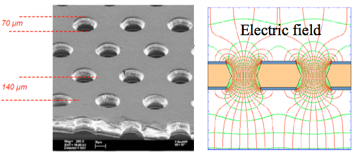
\includegraphics[width=12.0cm,height=5cm]{figures/GEM/KEKDTP3.jpg}
		\caption{(Left) The gas electron multiplier (GEM) foil can image two-dimensional position of particles passing through a gaseous chamber. (Right) The cross sectional view of the GEM shows strong electric fields in the vicinity of holes where electron signals are amplified.}
		\label{gem}
	\end{center}
\end{figure} 

The region inside {gem} detector consists of a drift electrode, a conversion and drift region, a {gem} mesh collecting and multiplying the charge in a gas avalanche, and induction gap in which a high electric field is used to extract and drift the electrons towards the collecting electrodes. This is shown in Figure \ref{gemgaps}. The large effective gains (up to $10^4$), full efficiency of detection and very good localization accuracies for minimum ionizing particles is promissing to us. In the thin gap of {gem} few tens of primary ion pairs creates; cascading to two {gem} meshes so it can provide large gains and better performances \cite{paper:2dgem}.
\begin{figure}[htb]
	\begin{center}
		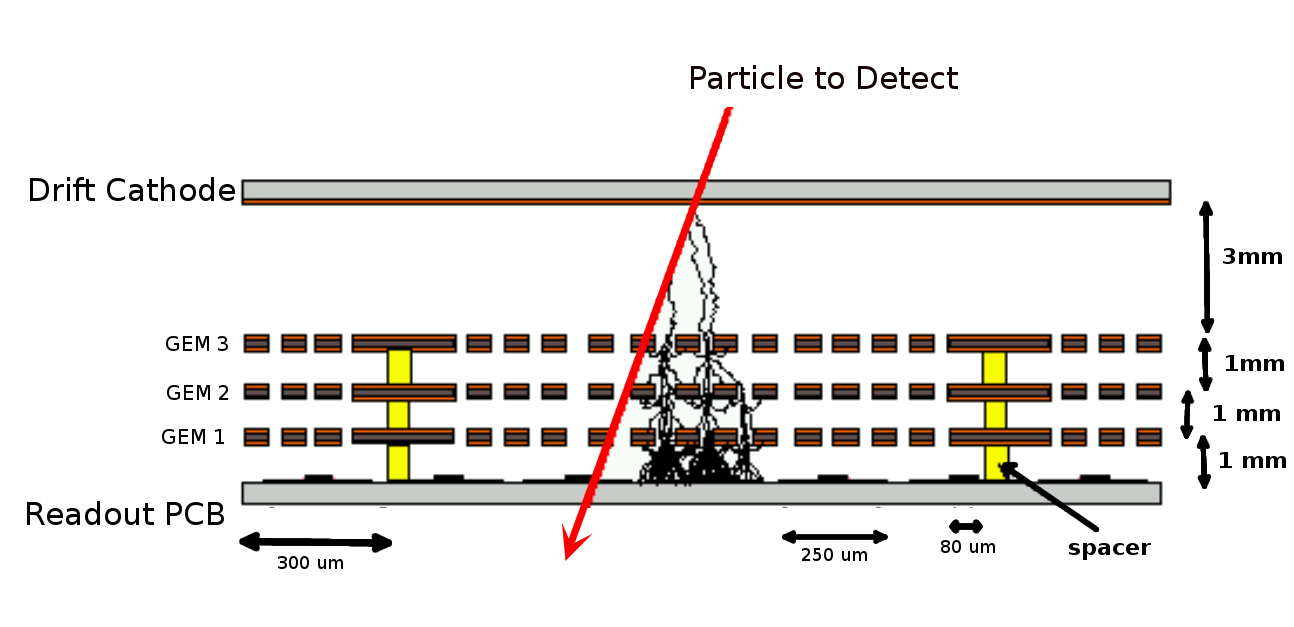
\includegraphics[width=10.0cm,height=7cm]{figures/GEM/triple_gem.png}
		\caption{Illustration of GEM working}
		\label{gemgaps}
	\end{center}
\end{figure} 

\section{GEM for CMS}
The CMS experiment was designed to have a highly redundant muon system using three detector technologies: {dt}, {csc} and {rpc}. The endcap regions rely on CSC and RPC for $|\eta|<1.6$. For higher $\eta~ (|\eta|>1.6)$ regions, the system has limited redundancy and only CSC are installed. In the future running of LHC at full luminosity, the particle rate in the forward region is expected to reach several tens of kHz/$cm^2$ and the integrated charge will reach several $C/cm^2$, which make the use of the originally planned RPC technology questionable. To overcome these limitations, the CMS GEM collaboration proposed the GEM as a potential candidate to upgrade the high-$\eta$ region of the forward muon system \cite{gemTDR}. 
%The CMS muon system was designed as a highly hermetic and redundant muon system, composed of three detection technologies. Precision measurements are provided by \gls{dt} in the barrel, covering acceptances up to $|\eta|<1.2$, and \gls{csc} in the endcaps covering $1.0 < |\eta|<2.4$. \gls{rpc} ensures adequate redundancy and triggering up to $\eta | > 1.6$ where the background particle rates are highest and the bending in the magnetic field is smallest.

The chosen technology are {gem}, where amplification occurs in the narrow wholes of a thin kapton foil. Three subsequent stages/foils allow for a reasonable amplification at every stage/foil while providing a high total amplification. Two of such triple-GEM chambers are combined to a so called super chamber.

The proposed upgrade targets the following improvements:
	\begin{itemize}
		\item Re-establish the redundancy in the difficult region beyond $\eta = 1.6 $;
		\item Improve tracking performance in the high rate environment;
		\item The combined operation of {csc} and {gem} detectors allows a measurement of the bending angle at trigger level, thus strongly reducing the rate of mis-measured muons driving the triggers rate.

	\end{itemize}

\section{Detector Design Description For Test Beam Analysis}
The full design of the GEM chamber is shown in Figure \ref{ge11}.
\begin{figure}[htb]
	\begin{center}
		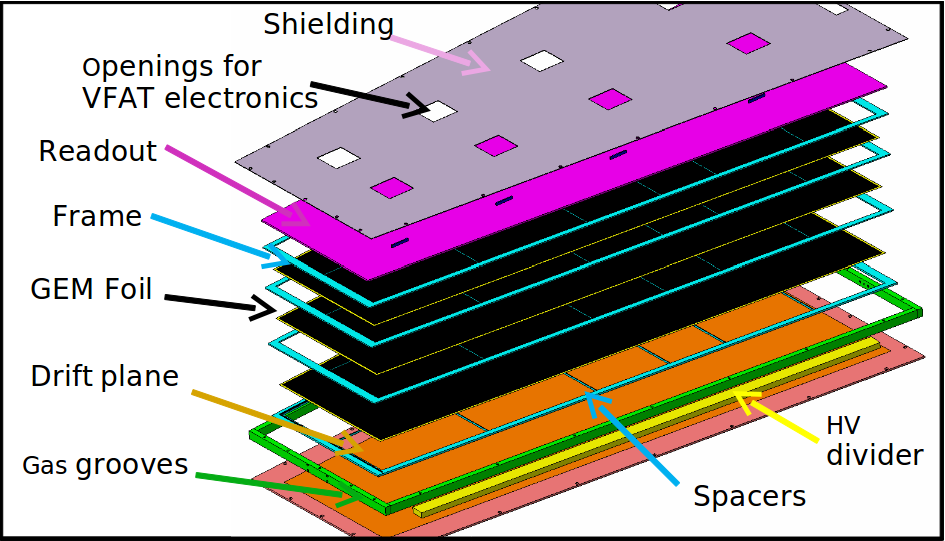
\includegraphics[width=10.0cm,height=7cm]{figures/GEM/ge11cad.png}
		\caption{Layer by layer view of GEM detector}
		\label{ge11}
	\end{center}
\end{figure} 
The trapezoidal chambers are sectorized in $\eta$ partitions to cover $10^0$ each in the azimuthal sector and provide radial readout strip with the strip pointing to the LHC beam pipe (Figure \ref{gemTrapezoidal}). In this design, the strip pitch varies from 0.6 mm (lower side) to 1.2 mm (upper side) with 8-$\eta$ sectors. To improve tracking capabilities, two GEM chambers will be mounted face-to-face to form a double layer called ``Super-Chamber". Thus each Super-Chamber will provide two impact points for each muon track. The gas gap configuration is: 3mm (drift), 1mm (transfer1), 2mm(transfer2), and 1mm (induction) as shown in Figure \ref{tripple-gem}, which proved to be optimal for timing purposes. The gas mixture is $Ar/CO_2/CF_4~45/15/40$.
\begin{figure}[htb]
	\begin{center}
		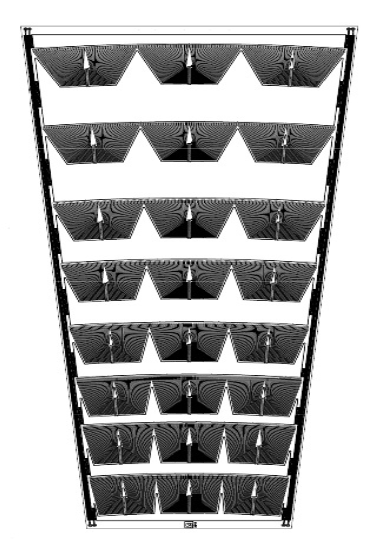
\includegraphics[width=6.0cm,height=12cm]{figures/GEM/gemTrapezoidal.png}
		\caption{Drawing of a large trapezoidal CMS GEM chamber showing $8-\eta$ partitions, each}
		\label{gemTrapezoidal}
	\end{center}
\end{figure} 
\begin{figure}[htb]
	\begin{center}
		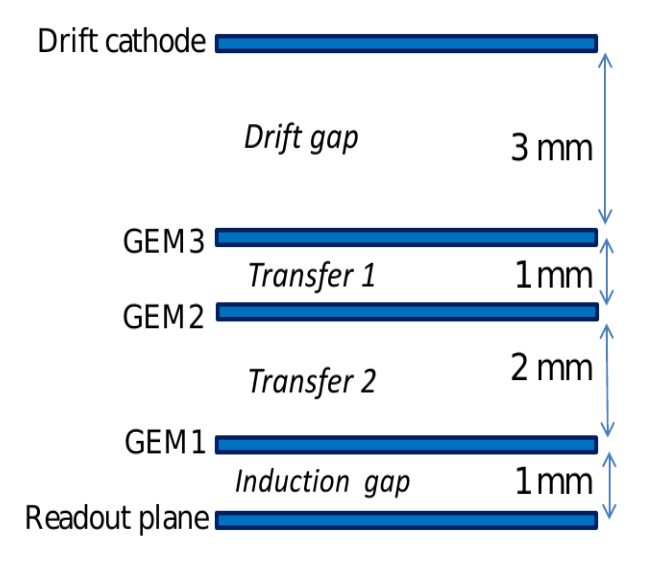
\includegraphics[width=8.0cm,height=6cm]{figures/GEM/tripple-gem.png}
		\caption{Cross-section of the proposed triple-GEM showing the dimensions of the different gaps}
		\label{tripple-gem}
	\end{center}
\end{figure} 
%The GEM production was achieved with the so called "Single-Mask" 
%\subsection{Test beam results}

Two large scale GEM chambers were tested at the SPS H2 beam line at CERN with 150GeV muon/pion beams. A hodoscope of small-area $(10\times 10 cm^2$) double sided GEM chambers was used to predict the hit position in the test chambers (Figure \ref{tbsetup}). Each tracking chamber has, on each side, 256 readout strips with a pitch of 0.4 mm.

\begin{figure}[htb]
	\begin{center}
		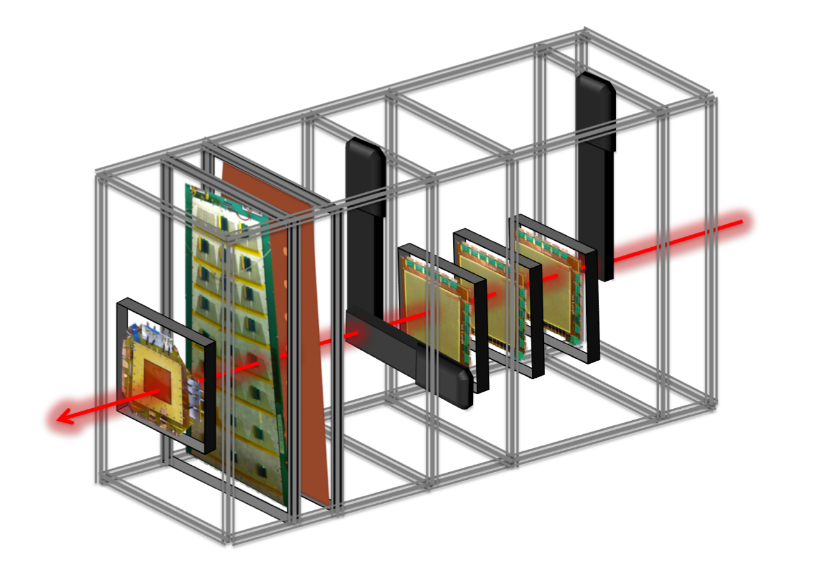
\includegraphics[width=8.0cm,height=6cm]{figures/GEM/tbsetup.png}
		\caption{Schematic view of the test beam setup with the three square GEM hodoscope and the trapezoidal CMS GEM chambers}
		\label{tbsetup}
	\end{center}
\end{figure} 

The full scale CMS GEM chamber has a trapezoidal shape with dimensions of $990\times (220-445)mm$. The strips are segmented in $8-\eta$ partitions. Each partition is sectorized along the $\phi$-coordinate into 3 readout sectors each with 128 strips. Thus 3072 channels are readout for the whole test chamber. During the test beam, two readout scenarios were used: digital TURBO/VFAT2 and Scalable Readout System (SRS) developed by RD51 collaboration and based on APV25 chips. The high voltage powering was realized using a ceramic high voltage divider. The CMS test chamber were placed, closed to the tracking hodoscope, on a vertically movable support to allow scanning. 

%Figure shows teh efficiency obtained


  % \newpage 
  \printbibliography
  % \printindex
  % \cleardoublepage
  % \printglossary[type=\acronymtype,title=Acronyms]


  % \appendix
  % \include{chapters/appendix1}

\end{document}